\section{Refitting the twin when the patient's normal beat changes}
\label{section:drift}

If the patient's normal beat changes after the twin was fitted, normal beats get high deviation scores and can be mistaken for abnormal ones. This section compares the Twin Calibration agent's three refitting policies (none, scheduled and drift; Section~\ref{section:twinClinical}).

\paragraph{Choosing $K$ and $H$.} We ran the agent with the drift policy on the training patients for four combinations of $K$ and $H$. Without any refits, 4.3\% of the normal beats had a score above 3. With $K = 0.5$ and $H = 40$ this fell to 1.9\%, with 1.9 refits per hour. $H = 20$ gave almost the same share (1.8\%) with 4.6 refits per hour, and $K = 1$ left more normal beats with high scores (2.3\%). We use $K = 0.5$ and $H = 40$. These runs also showed that the normal beat changes during several training recordings without any added change.

\paragraph{Experiment.} MIT-BIH does not tell us when a patient's normal beat changes, so we added a known change to the 21 test patients: between minute 10 and minute 25, the T wave of every beat (0.20--0.45~s after the R peak) is gradually turned over until it is inverted at half its original height, and it stays like that until the end of the recording. Each policy was run on the recordings with this change and, as a control, on the unchanged recordings. In both cases Arrhythmia Detection was replaced by the cardiologists' labels, so the results describe the twin's policy alone. For the normal beats we report the median score at the end of the recording and the share of scores above 3 after minute 10, i.e.\ normal beats that could be mistaken for abnormal ones (Table~\ref{tab:drift}).

\begin{table}[H]
\caption{Refitting policies on the test patients, with and without the added T-wave change. Normal beats only; refits do not include the first fit.}
\label{tab:drift}
\centering
\small
\setstretch{1.1}
\begin{tabular}{@{}llcccc@{}}
\toprule
\textbf{Recordings} & \textbf{Policy} & \textbf{\shortstack{Median score\\at the end}} & \textbf{\shortstack{Scores above 3\\after minute 10}} & \textbf{\shortstack{Refits per\\recording}} & \textbf{\shortstack{Alerts per\\recording}} \\
\midrule
unchanged & none & 1.13 & 5.6\% & 0 & 0 \\
 & scheduled & 1.04 & 5.2\% & 2.00 & 0 \\
 & drift & 1.04 & 2.3\% & 0.90 & 0.43 \\
\addlinespace
T wave inverted & none & 1.31 & 8.7\% & 0 & 0 \\
 & scheduled & 1.10 & 5.5\% & 2.00 & 0 \\
 & drift & 0.99 & 3.7\% & 1.05 & 0.48 \\
\bottomrule
\end{tabular}
\end{table}

\paragraph{Results.} Before minute 10 all policies give the same median score for normal beats (1.01). With the added change and no refits, the share of normal beats with a score above 3 rises from 5.6\% to 8.7\%. Refitting every 10 minutes lowers it to 5.5\% with two refits per recording; the drift policy lowers it to 3.7\% with about one refit per recording. The drift policy's first refit came a median of 430~s after the change began, because the change is gradual. On the unchanged recordings the drift policy also lowers the share, from 5.6\% to 2.3\%, since the normal beat already changes on its own in some recordings, while the scheduled policy barely helps (5.2\%). Figure~\ref{fig:drift} shows one recording.

\begin{figure}[H]
\centering
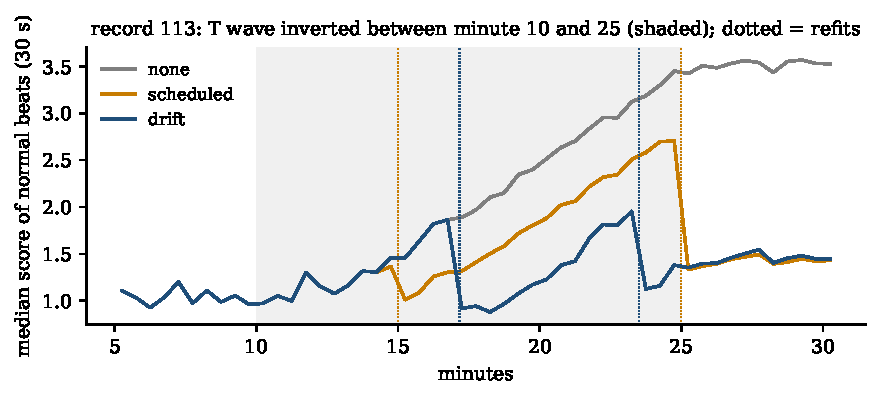
\includegraphics[width=0.88\textwidth]{Fig/s6_drift.pdf}
\caption{Record 113: median score of normal beats in 30~s steps. Shaded: the T wave is being inverted. Dotted lines: refits. Without refits the score keeps rising; the drift policy refits twice during the change, the scheduled policy at minutes 15 and 25.}
\label{fig:drift}
\end{figure}

\paragraph{Limitations.} How much the added change matters depends on the size of the patient's T wave in this lead. In record 100, for example, the T wave is so small that inverting it changes the beat by less than the patient's normal beat-to-beat variation. The results use the cardiologists' labels instead of the Detection agent and will be repeated once that agent is complete. Only one kind of change was tested.
